\documentclass{article}

% if you need to pass options to natbib, use, e.g.:
% \PassOptionsToPackage{numbers, compress}{natbib}
% before loading nips_2016
%
% to avoid loading the natbib package, add option nonatbib:
% \usepackage[nonatbib]{nips_2016}

%\usepackage[final]{nips_2016}
\usepackage{nips_2016}

% to compile a camera-ready version, add the [final] option, e.g.:
% \usepackage[final]{nips_2016}

\usepackage[utf8]{inputenc} % allow utf-8 input
\usepackage[T1]{fontenc}    % use 8-bit T1 fonts
\usepackage{hyperref}       % hyperlinks
\usepackage{url}            % simple URL typesetting
\usepackage{booktabs}       % professional-quality tables
\usepackage{amsfonts}       % blackboard math symbols
%\usepackage{nicefrac}       % compact symbols for 1/2, etc.
\usepackage{microtype}      % microtypography

\usepackage{amssymb, amsmath}
\usepackage{epsfig}
\usepackage{array}
\usepackage{ifthen}
\usepackage{color}
\usepackage{fancyhdr}
\usepackage{graphicx}
\usepackage{mathtools}
\usepackage{csquotes}
\usepackage{xcolor}
\usepackage{multirow}
\newcommand\crule[3][black]{\textcolor{#1}{\rule{#2}{#3}}}

\newcommand{\tr}{\text{tr}}
\newcommand{\E}{\textbf{E}}
\newcommand{\diag}{\text{diag}}
\newcommand{\argmax}{\text{argmax}}
\newcommand{\Cov}{\text{Cov}}
\newcommand{\Var}{\text{Var}}
\newcommand{\argmin}{\text{argmin}}
\newcommand{\Vol}{\text{Vol}}
\newcommand{\comm}[1]{}
\newcommand{\indep}{\rotatebox[origin=c]{90}{$\models$}}
\newcommand{\Cor}{\text{Cor}}

\definecolor{color1}{RGB}{128,13,13}
\definecolor{color2}{RGB}{70,128,13}
\definecolor{color3}{RGB}{13,128,128}
\definecolor{color4}{RGB}{70,13,128}

\title{Estimating mutual information in high dimensions via classification error}

% The \author macro works with any number of authors. There are two
% commands used to separate the names and addresses of multiple
% authors: \And and \AND.
%
% Using \And between authors leaves it to LaTeX to determine where to
% break the lines. Using \AND forces a line break at that point. So,
% if LaTeX puts 3 of 4 authors names on the first line, and the last
% on the second line, try using \AND instead of \And before the third
% author name.

\author{
  Charles Y.~Zheng \\
  Department of Statistics\\
  Stanford University\\
  Stanford, CA 94305 \\
  \texttt{snarles@stanford.edu} \\
  %% examples of more authors
  \And
  Yuval ~Benjamini \\
  Department of Statistics \\
  Hebrew University\\
  Jerusalem, Israel\\
  \texttt{yuval.benjamini@mail.huji.ac.il}
  %% Address \\
  %% \texttt{email} \\
  %% \AND
  %% Coauthor \\
  %% Affiliation \\
  %% Address \\
  %% \texttt{email} \\
  %% \And
  %% Coauthor \\
  %% Affiliation \\
  %% Address \\
  %% \texttt{email} \\
  %% \And
  %% Coauthor \\
  %% Affiliation \\
  %% Address \\
  %% \texttt{email} \\
}

\begin{document}
% \nipsfinalcopy is no longer used

\maketitle

\begin{abstract}
Estimating the mutual information $I(X; Y)$ based on observations
becomes statistically infeasible in high dimensions without some kind
of assumption or prior.  One approach is to assume a parametric joint
distribution on $(X, Y)$, but in many applications, such a strong
modeling assumption cannot be justified.  Alternatively, one can
estimate the mutual information based the performance of a classifier
trained on the data.  Existing methods include using the empirical
mutual information of the confusion matrix of the classifier, as well
as an estimator based on Fano's inequality.  However, both of these
methods all produce an estimate which is bounded by $\log(k)$, where
$k$ is the number of classes.  This presents a substantial limitation
for classification-based approaches, since the number of repeats per
class must be large for the classifier to work well, hence limiting
the number of classes $k$ that can be defined. In this paper, we
construct a novel classification-based estimator of mutual information
which overcomes these limitations.  Our estimator is based on
high-dimensional asymptotics: we show that in a particular limiting
regime, the mutual information is an invertible function of the
expected $k$-class Bayes error.  While the theory is based on a
large-sample, high-dimensional limit, we demonstrate through
simulations that our proposed lower confidence bound has superior
performance to the alternatives in problems of moderate
dimensionality.
\end{abstract}

\section{Introduction}

Mutual information $I(X; Y)$ is fundamentally a measure of dependence
between random variables $X$ and $Y$, and is defined as
\[
I(X;Y) = \int p(x, y) \log \frac{p(x, y)}{p(x)p(y)}dxdy.
\]
In its original context of information theory, the mutual information
describes the rate at which a noisy communications channel $Y$ can
communicate bits from a source stream $X$, but by now, the quantity
$I(X, Y)$ has found many new uses in science and engineering.  Mutual
information is used to test for conditional independence [1], to
quantifying the information between a random stimulus $X$ and the
signaling behavior of an ensembles of neurons, $Y$ [2]; for
use as an objective function for training neural networks [3], for
feature selection in machine learning, and even as an all-purpose
nonlinear measure of ``correlation for the 21st century'' [4].
What is common to all of these new applications, and what differs from
the original setting of Shannon's theory of information, is that the
variables $X$ and $Y$ have unknown distributions which must be
inferred from data.  In the case when $X$ and $Y$ are both
low-dimensional, for instance, when summarizing the properties of a
single neuron in response to a single stimulus feature, $I(X; Y)$ can
be estimated nonparametrically using a reasonable number of
observations.  There exists a huge literature on nonparametric
estimation of entropy and mutual information, see [5] for a
review.

However, the sample complexity for nonparametric estimation grows
exponentially with the dimension, rendering such methods ineffective
in applications with high-dimensional data [5].  One such
application includes multivariate pattern analysis (MVPA), an area of
neuroscience research pioneered by Haxby [6], which studies how
entire regions of the human brain respond to stimuli, using function
magnetic resonance imaging (fMRI) data; in MVPA studies, the input $X$
could be a natural image parameterized by $p = 10000$ image features,
while the output $Y$ is a $q=20000$-dimensional vector of brain
activation features obtained from the fMRI scan.  In problems of such
dimensionality, one can tractably estimate mutual information by
assuming a multivariate Gaussian model: however, this approach
essentially assumes a linear relationship between the input and
output, and hence fails to quantify nonlinear dependencies.  Rather
than assuming a full parametric generative model, one can empirically
select a good \emph{discriminative} model by using machine learning.
Treves [7] first proposed using the empirical mutual information of
the classification matrix in order to obtain a lower bound of the
mutual information $I(X; Y)$; this confusion-matrix-based lower bound
has subsequently enjoyed widespread use in the MVPA literature
[8].  But even earlier that this, the idea of linking
classification performance to mutual information can be found in the
beginnings of information theory: after all, Shannon's original
motivation was to characterize the minimum achievable error
probability of a noisy communication channel.  More explicitly, Fano's
inequality provides a lower bound on mutual information in relation to
the optimal prediction error, or Bayes error.  Therefore, one can
construct an estimator based on Fano's inequality, $\hat{I}_{Fano}$.
In either case, any method which derives an estimate of mutual
information from classification performance may be considered a
\emph{discriminative} estimation procedure, in contrast to the
\emph{parametric} and \emph{nonparametric} classes of estimation
procedures.

\subsection{Discriminative estimators of mutual information}

In many applications, the discriminative approach takes an
advantageous middle ground between the two extremes of nonparametric
and parametric approaches for estimating mutual information. In
neuroimaging data, we lack prior knowledge for specifying parametric
models, and the data is too high-dimensional for nonparametric
approaches, but we have a sufficient idea of the general ``structure''
in the data to achieve above-chance classification rates.

Five steps are required to implement discriminative estimation of
mutual information.  First, one must define a classification task.
The kinds of tasks that can be defined depend on the sampling scheme
used to collect the data.  Second, one chooses a classifier
$\mathcal{F}$.  Third, the classifier is trained on a training subset
of the data to obtain a classification rule $f$.  Fourthly, the
performance of the rule $f$ is evaluated on the held-out test set.
Finally, the performance metrics of the classifier are converted into
an estimate of mutual information.  In this paper we are mostly
concerned with the final step: how to convert measures of
classification performance into estimates of mutual information.

Let us assume that the variables $X, Y$ have a joint distribution $F$,
and that one can define a conditional distribution of $Y$ given $X$,
$Y|X \sim F_X,$ and let $G$ denote the marginal distribution of $X$.
We consider two different types of sampling procedures:
\begin{itemize}
\item \emph{pair sampling}: For $i = 1,\hdots, n$, the data $(X^i,
  Y^i)$ are sampled i.i.d. from the joint distribution of $(X, Y)$.
\item \emph{stratified sampling}: For $j = 1,\hdots, k$, sample
  i.i.d. \emph{exemplars} $X^{(1)},\hdots, X^{(k)} \sim G$.  For $i =
  1,\hdots, n$, draw $Z^i$ iid from the uniform distribution on
  $1,\hdots, k$, then draw $Y^i$ from the conditional distribution
  $F_{X^{(Z_i)}}$.
\end{itemize}

Pair sampling occurs in observational studies, where one observes both
$X$ and $Y$ externally.  On the other hand, stratified sampling is
more commonly seen in controlled experiments, where an experimenter
chooses an input $X$ to feed into a black box, which outputs $Y$.  An
example from fMRI studies is an experimental design where the subject
is presented a stimulus $X$, and the experimenter measures the
subject's response via the brain activation $Y$. \footnote{Note the
  asymmetry in our definition of stratified sampling: our convention
  is to take $X$ to be the variable preceding $Y$ in causal order.
  Such causal directionality constrains the stratified sampling to
  have repeated $X$ rather than repeated $Y$ values, but has no
  consequence for the mutual information $I(X; Y)$, which is a
  symmetric function.}

Given data from either pair sampling or stratified sampling, one can
define various \emph{classification tasks}.  Here, the point is to use
classification as a tool for extracting information about the
relationship between $X$ and $Y$.  As such, it is up to us to define
the classification tasks of interest.  For instance, one can define
tasks which either classify $Y$ based on $X$, or classify $X$ based on
$Y$; without loss of generality, we henceforth consider the latter.
In the case of continuous $X$, we can define an arbitrary number of
classes $k$ by specifying a partition on the space of $X$.  That is,
one can define a \emph{class function} $Z: X \to \{1,\hdots, k\}$, and
consider the problem of classifying $Z$ given $Y$.  A classification
rule is any (possibly stochastic) mapping $f: \mathcal{Y} \to
\{1,\hdots, k\}$, where $\mathcal{Y}$ is a superset of the support of
$Y$.  The \emph{generalization error} of the classification rule is $
e_{gen}(f) = Pr[f(Y) \neq Z].  $ The Bayes error is the generalization
error of the optimal classification rule, $ e_{Bayes}(f) = \inf_f
e_{gen}(f) $ We call such a classification task a
\emph{partition-based} classification task.

The freedom to choose the partition $Z$ may be more of a curse than a
blessing when it is unclear how to choose an appropriate partition on
the support of $X$.  If stratified sampling is employed, one can
define an \emph{exemplar-based} classification task which avoids
having to specify a partition.  One defines the \emph{class function}
$Z$ by
\[
Z: \{X^{(1)}, \hdots, X^{(k)}\} \to \{1,\hdots, k\},
\]
\[
Z(X^{(i)}) = i\text{ for }i = 1, \hdots, k.
\]
Note that the domain of $Z$ is restricted to the set of observed
exemplars $X^{(1)},\hdots, X^{(k)}$.  The loss function is not
well-defined when $X$ lies outside the set of exemplars, so it is
natural to define the generalization error by
\begin{equation}\label{egendef}
e_{gen}(f) = \frac{1}{k} \sum_{i=1}^k\Pr[f(Y) \neq Z|X = X^{(i)}].
\end{equation}
Indeed, in experiments where stratified sampling is used, this is the
most commonly employed notion of generalization error [9].  
In an exemplar-based classification, there is no need to
specify an arbitrary partition on the input space, but now the $k$
classes will now be \emph{randomly} defined.  One consequence is that
the Bayes error $e_{Bayes}$ is a random variable: when the sampling
produces $k$ similar exemplars, $e_{Bayes}$ will be higher, and when
the sampling produces well-separated exemplars $e_{Bayes}$ may be
lower.  Therefore, in stratified sampling, it is useful to consider
the \emph{average Bayes error},
\begin{equation}\label{abedef}
e_{ABE, k} = \E_{X^{(1)},\hdots, X^{(k)}}[e_{Bayes}],
\end{equation}
where the expectation is taken over the joint distribution of
$X^{(1)},\hdots, X^{(k)} \stackrel{iid}{\sim} G$.

Unless expert knowledge is available, it is usually necessary to
choose the function $f$ in a data-dependent way in order to obtain a
reasonable classification rule.  We use the terminology
\emph{classifier} to refer to any algorithm which takes data as input,
and produces a classification rule $f$ as output.  Mathematically
speaking, the classifier is a functional which maps a set of
observations to a classification rule, $ \mathcal{F}:
\{(x^{1},y^{1}),\hdots, (x^{m}, y^{m})\} \mapsto f(\cdot).  $ The data
$(x^1,y^1),\hdots, (x^m, y^m)$ used to obtain the classification rule
is called \emph{training data.}  When the goal is to obtain
\emph{inference} about the generalization error $e_{gen}$ of the
classification rule $f$, it becomes necessary to split the data into
two independent sets: one set to train the classifier, and one to
evaluate the performance.  The reason that such a splitting is
necessary is because using the same data to test and train a
classifier introduces significant bias into the empirical
classification error [10].  One creates a
\emph{training set} consisting of $r_1$ repeats per class, $ S_{train}
= \{(x^{(i)}, y^{(i),j})\}_{i=1, j=1}^{k, r_1}, $ and a \emph{test
  set} consisting of the remaining $r_2 = r - r_1$ repeats, $ S_{test}
= \{(x^{(i)}, y^{(i),j})\}_{i=1, j=r_1}^{k, r}.  $ The classification
rule is obtained via $ f = \mathcal{F}(S_{train}), $ and the
performance of the classifier is evaluated by predicting the classes
of the test set.  The results of this test are summarized by a $k
\times k$ \emph{confusion matrix} $M$ with $ M_{ij} = \sum_{\ell=r_1 +
  1}^r I(f(y^{(i), r}) = j).  $ The $i, j$th entry of $M$ counts how
many times a output in the $i$th class was classified to the $j$th
class.  The \emph{test error} is the proportion of off-diagonal terms
of $M$, $ e_{test} = \frac{1}{kr} \sum_{i \neq j} M_{ij}, $ and is an
unbiased estimator of $e_{gen}$.  However, in small sampling regimes
the quantity $e_{test}$ may be too variable to use as an estimator of
$e_{gen}$.  We recommend the use of Bayesian smoothing, defining an
$\alpha$-smoothed estimate $\hat{e}_{gen, \alpha}$ by $ \hat{e}_{gen,
  \alpha} = (1 - \alpha) e_{test} + \alpha \frac{k-1}{k}, $ which
takes a weighted average of the unbiased estimate $e_{test}$, and the
natural prior of \emph{chance classification}.

We define a discriminative estimator to be a function which maps the
misclassification matrix to a positive number, $ \hat{I}:
\mathbb{N}^{k \times k} \to \mathbb{R}.  $ We are aware of the
following examples of discriminative estimators: (1) estimators
derived from using Fano's inequality, and (2) the empirical
information of the confusion matrix, as introduced by Treves [7].

Fano's inequality can be easily adapted to yield a discriminative
estimator.  The original inequality reads
\[
H(Z|Y) \leq H(e_{Bayes}) + e_{Bayes} \log ||\mathcal{Z}| - 1|
\]
where $H(e)$ is the entropy of a Bernoulli random variable with
probability $e$.  Replacing $H(Z|Y)$ with $H(X|Y)$ and replacing
$e_{Bayes}$ with $\hat{e}_{gen, \alpha}$, we get the estimator
\[
\hat{I}_{Fano}(M) = log(K) - \hat{e}_{gen, \alpha} log(K-1) + \hat{e}_{gen, \alpha} log(p) + (1-\hat{e}_{gen, \alpha}) log(1-\hat{e}_{gen, \alpha}).
\]
Meanwhile, the confusion matrix estimator computes
\[
\hat{I}_{CM}(M) = \frac{1}{k^2} \sum_{i=1}^k \sum_{j=1}^k \log \frac{M_{ij}}{r/k},
\]
which is the empirical mutual information of the discrete joint
distribution $(Z, f(Y))$.

As noted in the literature [8], such discriminative
approaches tend to underestimate the mutual information.  Two sources
of ``information loss'' are (1) the fact that a continuous input
variable $X$ is discretized into $k$ classes, and (2) that the
performance of any classifier trained from data can at best given an
\emph{upper bound} to the error of the best classification rule: the
Bayes error.  Dealing with the problem of estimating the Bayes error
is beyond the scope of the current paper, but we will argue that the
stratified sampling design overcomes some of the limitations imposed
by the discretization of $X$.

\subsection{The problem of undersampling}

Stratified sampling is commonly used in neuroscience experiments, and
furthermore, it is often the case that the number of classes $k$ is
constrained to be small due to practical and statistical
considerations [11].  When $\log(k) \ll I(X; Y)$, we say
that the data is \emph{undersampled}: meaning that even if the total
number of observations is large (due to having many repeats per
class,) the diversity of the exemplar set is poor.

The parametric approach is relatively robust to undersampling of the
exemplars, since $k$ exemplars suffice to identify a $p < k$-parameter
model.  Gastpar et al. [11], studied the nonparametric estimator
\[
\hat{I}_0 = \hat{H}(Y) - \frac{1}{k}\sum_{i=1}\hat{H}(Y|X^{(i)}),
\]
where $\hat{H}$ is an estimator for the entropy.  Gastpar et
al. showed that $\hat{I}_0$ is biased downwards due to undersampling
of the exemplars: to counteract this bias, they introduce the
anthropic correction estimator $\hat{I}_\alpha$.  However, without a
principled approach to choose the parameter $\alpha \in (0,1]$,
  $\hat{I}_\alpha$ could still vastly underestimate or overestimate
  the mutual information.

Meanwhile, the discriminative estimators $\hat{I}_{CM}$ and
$\hat{I}_{Fano}$ perform quite badly in the undersampled regime.  It
is easy to show that $\log(k)$ is a tight upper bound for both
$\hat{I}_{CM}$ and $\hat{I}_{Fano}$.  As $I(X; Y)$ exceeds $\log(k)$,
the estimate $\hat{I}$ can no longer approximate $I(X; Y)$, even up to
a constant factor.  On the other hand, the following worst-case
example shows that discriminative estimators cannot overcome this
$\log(k)$ barrier in general.  Let $X$ and $Y$ have joint density $
p(x, y) = \frac{1}{k}I(\lfloor kx \rfloor = \lfloor ky \rfloor) $ on
the unit square.  Under partition-based classification, if we set
$Z(x) = \lfloor kx \rfloor + 1$, then no errors are made under the
Bayes rule. We therefore have a joint distribution which maximizes any
reasonable discriminative estimator but has \emph{finite} information
$I(X; Y) = \log(k)$.  The consequence of this is that under
partition-based classification, we cannot hope to distinguish
distributions with $I(X; Y) > \log(k)$.  The situation is more
promising if we specialize to stratified sampling: in the same
example, a Bayes of zero is no longer likely due to the possibility of
exemplars being sampled from the same bin (`collisions')--we obtain an
approximation to the average Bayes error through a Poisson sampling
model: $e_{ABE, k} \approx \frac{1}{e}\sum_{j=1}^\infty
\frac{1}{j(j!)}= 0.484$.  Recognizing that the natural setting for
discriminative estimation is for high-dimensional data, we specialize
further to consider deriving an estimator under a
\emph{high-dimensional} regime.  The extra assumption of high
dimensionality allows an extreme degree of control over the average
Bayes error--it reduces the average Bayes error to a function of the
mutual information!

In section 2 we present an asymptotic setting intended to capture the
notion of high dimensionality; namely, one where the number of classes
is fixed, and where the information $I(X; Y)$ remains fixed, while the
dimensionality of the input $X$ and output $Y$ both grow to infinity.
We make a number of additional regularity conditions to rule out
scenarios where $(X, Y)$ is really less ``high-dimensional'' than it
appears, since most of the variation is captured a low-dimensional
manifold\footnote{In situations where $(X, Y)$ lie on a manifold, one
  could effectively estimate mutual information by would be to
  combining dimensionality reduction with nonparametric information
  estimation [12]. }.  In section 2.1 we
present our key result, which links the asymptotic average Bayes error
to the mutual information; in section 2.2 we apply this result to
derive our proposed estimator, $\hat{I}_{HD}$ (where HD stands for
``high-dimensional.'')  Section 3 presents simulation results, and
section 4 concludes.  All proofs are given in the supplement.

\section{Theory}

We derive a new discriminative estimator by exploiting the properties
of stratified sampling, plus a universality property that arises in
high-dimensions.  This universality phenomenon allows us to establish
a relationship between the mutual information $I(X; Y)$ and the
$k$-class average Bayes error, $e_{ABE, k}$.  In short, we will
identify a function $\pi_k$ (which depends on $k$),
\begin{equation}\label{abepi}
e_{ABE, k} \approx \pi_k(\sqrt{2 I(X; Y)})
\end{equation}
and that this approximation becomes accurate under a limit where $I(X;
Y)$ is small relative to the dimensionality of $X$, and under the
condition that the components of $X$ are approximately independent.
The function $\pi_k$ is given by
\[
\pi_k(c) = 1 - \int_{\mathbb{R}} \phi(z - c)  \Phi(z)^{k-1} dz.
\]
This formula is not new to the information theory literature: it
appears as the error rate of an orthogonal constellation [13].  What
is surprising is that the same formula can be used to approximate the
error rate in much more general class of classification
problems\footnote{An intuitive explanation for this fact is that
  points from any high-dimensional distribution lie in an orthogonal
  configuration with high probability.}--this is precisely the
universality result which provides the basis for our proposed
estimator.

Figure \ref{fig:pi} displays the plot of $\pi_k$ for several values of
$k$.  For all values of $k$, $\pi_k(\mu)$ is monotonically decreasing
in $\mu$, and tends to zero as $\mu \to \infty$, which is what we
expect since if $I(X; Y)$ is large, then the average Bayes error
should be small.  Another intuitive fact is that $ \pi_k(0) = 1 -
\frac{1}{k}, $ since after all, an uninformative response cannot lead
to above-chance classification accuracy.

\begin{figure}
\centering
\begin{tabular}{ccrl}
\multirow{5}{*}{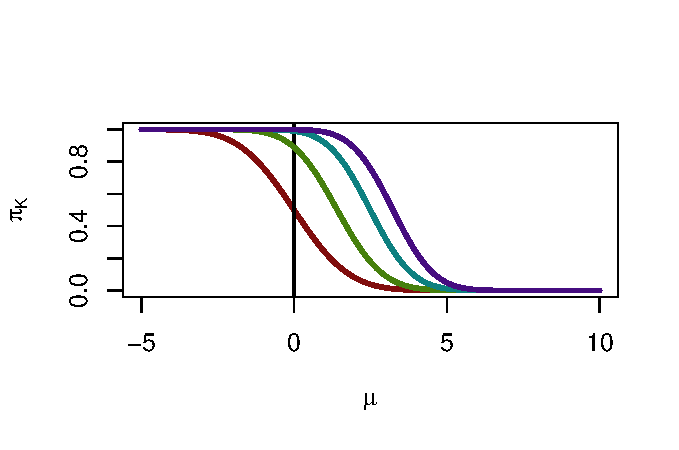
\includegraphics[scale = 0.5, clip=true, trim=0 0.2in 0 0.5in]{../info_theory_sims/illus_piK_flat.pdf}} &
\multirow{5}{*}{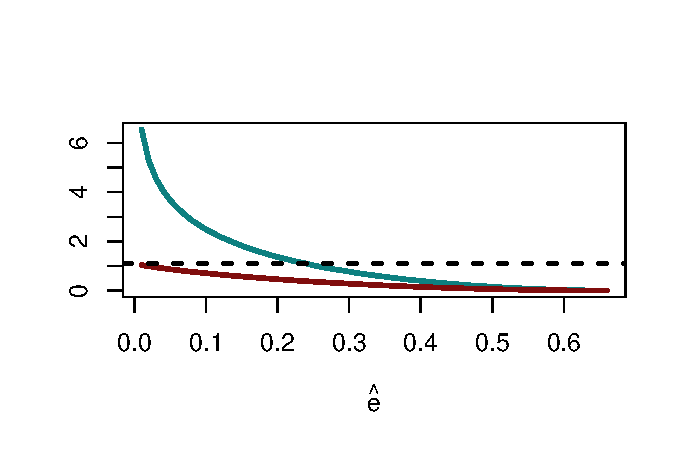
\includegraphics[scale = 0.5, clip=true, trim=0 0.2in 0.4in 0.5in]{../info_theory_sims/ihat_comp.pdf}} & & \\
& & & \\
& & \crule[color1]{0.2cm}{0.2cm} & $\hat{I}_{Fano}$\\
& & \crule[color3]{0.2cm}{0.2cm} & $\hat{I}_{HD}$\\
& & & \\
& & & \\
& & & \\
& & & 
\end{tabular}
\caption{Left: The function $pi_k(\mu)$ for $k = \{2, 10\}$.
Right: $\hat{I}_{HD}$ with $\hat{I}_{Fano}$ as functions of $\hat{e}_{gen}$, for $k = 3$.
While $\hat{I}_{Fano}$ is bounded from above by $\log(k)$ (dotted line), $\hat{I}_{HD}$ is unbounded.
\label{fig:pi}}
\end{figure}

\subsection{Universality result}

We obtain the universality result in two steps.  First, we link the
average Bayes error to the moments of some statistics $Z_i$.
Secondly, we use taylor approximation in order to express $I(X; Y)$ in
terms of the moments of $Z_i$.  Connecting these two pieces yields the
formula \eqref{abepi}.

Let us start by rewriting the average Bayes error:
\[
e_{ABE, k} = \Pr[p(Y|X_1) \leq \max_{j \neq 1} p(Y|X_j)| X = X_1].
\]
Defining the statistic $Z_i = \log p(Y|X_i) - \log p(Y|X_1)$, where $Y
\sim p(y|X_1)$, we obtain $ e_{ABE} = \Pr[\max_{j > 1} Z_i > 0].  $
The key assumption we need is that $Z_2,\hdots, Z_k$ are
asymptotically multivariate normal.  If so, the following lemma allows
us to obtain a formula for the misclassification rate.

\textbf{Lemma 1. }
\emph{
Suppose $(Z_1, Z_2, \hdots, Z_k)$ are jointly multivariate normal, with 
$\E[Z_1 - Z_i]= \alpha$, 
$\Var(Z_1) = \beta \geq 0$, 
$\Cov(Z_1, Z_i) = \gamma$, 
$\Var(Z_i)= \delta$, and $\Cov(Z_i, Z_j) = \epsilon$ for all $i, j = 2, \hdots,
k$, such that $\beta + \epsilon - 2\gamma > 0$.  Then, letting
\[
\mu = \frac{\E[Z_1 - Z_i]}{\sqrt{\frac{1}{2}\Var(Z_i - Z_j)}} = \frac{\alpha}{\sqrt{\delta - \epsilon}},
\]
\[
\nu^2 = \frac{\Cov(Z_1 -Z_i, Z_1 - Z_j)}{\frac{1}{2}\Var(Z_i - Z_j)} = \frac{\beta + \epsilon - 2\gamma}{\delta - \epsilon},
\]
we have
\begin{align*}
\Pr[Z_1 < \max_{i=2}^k Z_i] &= \Pr[W < M_{k-1}]
\\&= 1 - \int \frac{1}{\sqrt{2\pi\nu^2}} e^{-\frac{(w-\mu)^2}{2\nu^2}} \Phi(w)^{k-1} dw,
\end{align*}
where $W \sim N(\mu, \nu^2)$ and $M_{k-1}$ is the maximum of $k-1$
independent standard normal variates, which are independent of $W$.
}

To see why the assumption that $Z_2,\hdots, Z_k$ are multivariate normal might be justified, suppose that $X$ and $Y$ have the same dimensionality $d$, and that
joint density factorizes as
\[
p(x^{(j)}, y) = \prod_{i=1}^d p_i(x^{(j)}_i, y_i)
\]
where $x_i^{(j)}, y_i$ are the $i$th scalar components of the vectors $x^{(j)}$ and $y$.
Then,
\[
Z_i = \sum_{m=1}^d \log p_m(y_m | x^{(i)}_m) - \log p_m(y_m | x^{(m)}_1)
\]
where $x_{i, j}$ is the $i$th component of $x_j$.  The $d$ terms $\log
p_m(y_m | x_{m, i}) - \log p_m(y_m | x_{m, 1})$ are independent across
the indices $m$, but dependent between the $i = 1,\hdots, k$.
Therefore, the multivariate central limit theorem can be applied to
conclude that the vector $(Z_2,\hdots, Z_k)$ can be scaled to converge
to a multivariate normal distribution.  While the componentwise
independence condition is not a realistic assumption, the key property
of multivariate normality of $(Z_2,\hdots, Z_k)$ holds under more
general conditions, and appears reasonable in practice.

It remains to link the moments of $Z_i$ to $I(X;Y)$.  This is accomplished by approximating the logarithmic term by the Taylor expansion
\[
\log \frac{p(x, y)}{p(x) p(y)} \approx \frac{p(x, y) - p(x) p(y)}{p(x) p(y)} - \left(\frac{p(x, y) - p(x) p(y)}{p(x) p(y)}\right)^2 + \hdots.
\]
A number of assumptions are needed to ensure that needed
approximations are sufficiently accurate; and additionally, in order
to apply the central limit theorem, we need to consider a
\emph{limiting sequence} of problems with increasing dimensionality.
We now state the theorem.

\textbf{Theorem 1.} \emph{Let $p^{[d]}(x, y)$ be a sequence of joint densities
for $d = 1,2,\hdots$.  Further assume that
\begin{itemize}
\item[A1.] $\lim_{d \to \infty} I(X^{[d]}; Y^{[d]}) = \iota < \infty.$
\item[A2.] There exists a sequence of scaling constants $a_{ij}^{[d]}$
and $b_{ij}^{[d]}$ such that the random vector $(a_{ij}\ell_{ij}^{[d]} +
b_{ij}^{[d]})_{i, j = 1,\hdots, k}$ converges in distribution to a
multivariate normal distribution.
\item[A3.] Define \[
u^{[d]}(x, y) = \log p^{[d]}(x, y) - \log p^{[d]}(x) - \log p^{[d]}(y).
\]
There exists a sequence of scaling constants $a^{[d]}$, $b^{[d]}$ such that
\[
a^{[d]}u^{[d]}(X^{(1)}, Y^{(2)}) + b^{[d]}
\]
converges in distribution to a univariate normal distribution.
\item[A4.] For all $i \neq k$,
\[\lim_{d \to \infty}\Cov[u^{[d]}(X^{(i)}, Y^{(j)}), u^{[d]}(X^{(k)}, Y^{(j)})] = 0.\]
\end{itemize}
Then for $e_{ABE, k}$ as defined above, we have
\[
\lim_{d \to \infty} e_{ABE, k} = \pi_k(\sqrt{2 \iota})
\]
where
\[
\pi_k(c) = 1 - \int_{\mathbb{R}} \phi(z - c)  \Phi(z)^{k-1} dz
\]
where $\phi$ and $\Phi$ are the standard normal density function and
cumulative distribution function, respectively.}

Assumptions A1-A4 are satisfied in a variety of natural models.  One
example is a multivariate Gaussian sequence model where $X \sim N(0,
\Sigma_d)$ and $ Y = X + E $ with $ E \sim N(0, \Sigma_e), $ where
$\Sigma_d$ and $\Sigma_e$ are $d \times d$ covariance matrices, and
where $X$ and $E$ are independent.  Then, if $d \Sigma_d$ and
$\Sigma_e$ have limiting spectra $H$ and $G$ respectively, the joint
densities $p(x, y)$ for $d = 1,\hdots, $ satisfy assumptions A1 - A4.
Another example is the multivariate logistic model, which we describe
in section 3.  We further discuss the rationale behind A1-A4 in the
supplement, along with the detailed proof.

\subsection{High-dimensional estimator}

The estimator we propose is
\[
\hat{I}_{HD}(M) = \frac{1}{2}(\pi_{k}^{-1}(\hat{e}_{gen, \alpha}))^2,
\]
obtained by inverting the relation \eqref{abepi}, then substituting
the estimate $\hat{e}_{gen, \alpha}$ for the $e_{ABE, k}$.  As such,
our estimator can be directly compared to the $\hat{I}_{Fano}$, since
both are functions of $\hat{e}_{gen,\alpha}$ (Figure 1.)

For sufficiently high-dimensional problems, $\hat{I}_{HD}$ can
accurately recover $I(X; Y) > \log k$, supposing also that the
classifier $\mathcal{F}$ consistently estimates the Bayes rule.  The
number of observations needed depends on the convergence rate of
$\mathcal{F}$ and also the complexity of estimating $e_{gen, \alpha}$.
Therefore, without making assumptions on $\mathcal{F}$, the sample
complexity is at least exponential in $I(X; Y)$.  This is because when
$I(X; Y)$ is large relative to $\log(k)$, the Bayes error $e_{ABE, k}$
is exponentially small.  Hence $O(1/e_{ABE, k})$ observations in the
test set are needed to recover $e_{ABE, k}$ to sufficient precision.
While the sample complexity exponential in $I(X; Y)$ is by no means
ideal, by comparison, the nonparametric estimation approaches have a
complexity exponential in the dimensionality.  Hence, $\hat{I}_{HD}$
is favored over nonparametric approaches in settings with high
dimensionality and low signal-to-noise ratio.


\section{Simulation}

We compare the discriminative estimators $\hat{I}_{CM}$,
$\hat{I}_{Fano}$, $\hat{I}_{HD}$ with a nonparametric estimator
$\hat{I}_0$ in the following simulation.  We generate data according
to a multiple-response logistic regression model, where $ X \sim N(0,
I_p) $, and $Y$ is a binary vector with conditional distribution
\[
Y_i|X = x \sim \text{Bernoulli}(x^T B_i)
\]
where $B$ is a $p \times q$ matrix.  One application of this model
might be modeling neural spike count data $Y$ arising in response to
environmental stimuli $X$ [14].  We choose the naive Bayes for the
classifier $\mathcal{F}$: it is consistent for estimating the Bayes
rule.  In Figure 2 we show the sampling distributions of the four
estimators as $I(X; Y)$ is varied in the interval $[0, 4]$.  We see
that $\hat{I}_{CM}$, $\hat{I}_{Fano}$, and $\hat{I}_0$ indeed begin to
asymptote as they approach $\log(k) = 2.995$.  In contrast,
$\hat{I}_{HD}$ remains a good approximation of $I(X; Y)$ within the
range, although it begins to overestimate at the right endpoint.

\begin{figure}
\begin{center}
\begin{tabular}{ccrl}
&\multirow{10}{*}{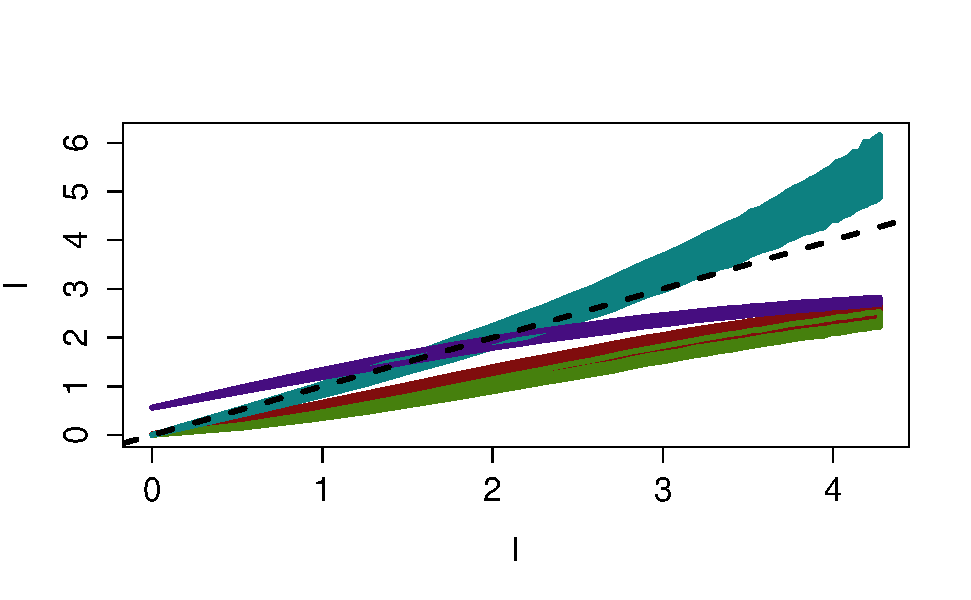
\includegraphics[scale = 0.5, clip=true, trim=0.4in 0.5in 0 0.5 in]{../info_theory_sims/fig4.pdf}}&&\\
&  $I(X; Y)$& &\\
& & &\\
& & &\\
& & \crule[color3]{0.2cm}{0.2cm} &$\hat{I}_{HD}$\\
 & &\crule[color1]{0.2cm}{0.2cm} &$\hat{I}_{CM}$ \\
$\hat{I}$& & \crule[color2]{0.2cm}{0.2cm} &$\hat{I}_{Fano}$\\
& & \crule[color4]{0.2cm}{0.2cm} &$\hat{I}_{0}$\\
& & &\\
& & &\\
& & &\\
\end{tabular}
\end{center}
\caption{Sampling distributions of $\hat{I}$ for data generated from the multiple-response logistic model.  $p = q = 10$; $k= 20$; $B = sI_{10}$, where $s \in [0, \sqrt{200}]$; and  $r = 1000$.}
\end{figure}

\section{Discussion}

Discriminative estimators of mutual information have the potential to
estimate mutual information in high-dimensional data without resorting
to fully parametric assumptions.  However, a number of practical
considerations also limit their usage.  First, one has to find a good
classifier $\mathcal{F}$ for the data: techniques for model selection
can be used to choose $\mathcal{F}$ from a large library of methods.
However, there is no way to guarantee how well the chosen classifier
approximates the optimal classification rule.  Secondly, one has to
estimate the generalization error from test data: the complexity of
estimating $e_{gen}$ could become the bottleneck when $e_{gen}$ is
close to 0.  Thirdly, for previous estimators $\hat{I}_{Fano}$ and
$\hat{I}_{CM}$, the ability of the estimator to distinguish high
values of $I(X; Y)$ is limited by the number of classes $k$.  Our
estimator $\hat{I}_{HD}$ is subject to the first two limitations,
along with any conceivable discriminative estimator, but overcomes the
third limitation under the assumption of stratified sampling and high
dimensionality.

While the high-dimensionality assumption is well-suited for a broad
class of applications, the stratified sampling assumption can be
justified only in certain types of controlled experiments.  On the
other hand, the stratified sampling assumption may not be essential to
our approach: we use it mainly as a mathematical convenience.
Therefore, it remains a possibility to extend the proposed estimation
approach to handle partition-based classification, under certain
assumptions on the partition.

As it stands, a number of adjustments can be made to $\hat{I}_{HD}$ to
improve its performance in special cases.  One can employ more
sophisticated methods to estimate $e_{ABE, k}$: for example,
extrapolating from learning curves [15].  Furthermore,
depending on the risk function, one may debias or shrink the estimate
$\hat{I}_{HD}$ to achieve a more favorable bias-variance tradeoff.

In our simulation experiment, our proposed estimator is seen to
outperform existing estimators, but it remains to assess the utility
of our estimation procedure in a real-world example.  In a forthcoming
work, we apply our framework to evaluate visual encoding models in
human fMRI data.


\subsubsection*{Acknowledgments}

CZ is supported by an NSF graduate research fellowship.

\section*{References}

\small

[1] De Campos, Luis M. ``A scoring function for learning Bayesian networks
based on mutual information and conditional independence tests." \emph{The
Journal of Machine Learning Research 7} (2006): 2149-2187.

[2] Borst, A. \& Theunissen, F. E. ``Information theory and neural coding''
\emph{Nature Neurosci.}, vol. 2, pp. 947?957, Nov. 1999.

[3] Linsker, Ralph. ``An application of the principle of maximum
information preservation to linear systems." \emph{Advances in neural
information processing systems.} 1989.

[4] Speed, Terry. "A correlation for the 21st century." \emph{Science}
334.6062 (2011): 1502-1503.

[5] Beirlant, J., Dudewicz, E. J., Gy\:{o}rfi, L., \& der Meulen,
E. C. (1997). ``Nonparametric Entropy Estimation: An
Overview.'' \emph{International Journal of Mathematical and Statistical
Sciences}, 6, 17–40. doi:10.1.1.87.5281

[6] Haxby, James V., et al. "Distributed and overlapping representations of faces and objects in ventral temporal cortex." \emph{Science} 293.5539 (2001): 2425-2430.

[7] Treves, A. (1997). ``On the perceptual structure of face space.'' \emph{Bio Systems}, 40(1-2), 189?96. 

[8] Quiroga, Q. R., \& Panzeri, S. (2009). Extracting information from neuronal populations: information theory and decoding approaches. \emph{Nature Reviews. Neuroscience}, 10(3), 173?185.

[9] Naselaris, T., Kay, K. N., Nishimoto, S., \& Gallant,
J. L. (2011). Encoding and decoding in fMRI. \emph{Neuroimage}, 56(2),
400-410.

[10] Friedman, J., Hastie, T., \& Tibshirani, R. \emph{The elements
of statistical learning.} Vol. 1. Springer, Berlin: Springer series in
statistics, 2008.

[11] Gastpar, M.  Gill, P.  Huth, A. \& Theunissen, F. ``Anthropic
Correction of Information Estimates and Its Application to Neural
Coding.'' \emph{IEEE Trans. Info. Theory}, Vol 56 No 2, 2010.

[12] Theunissen, F. E. \& Miller, J.P. ``Representation of sensory
information in the cricket cercal sensory system. II. information
theoretic calculation of system accuracy and optimal tuning-curve
widths of four primary interneurons,'' \emph{J. Neurophysiol.}, vol. 66,
no. 5, pp. 1690-1703, 1991.

[13] Tse, D., \& Viswanath, P. \emph{Fundamentals of wireless
communication.} Cambridge university press, 2005.

[14] Banerjee, A., Dean, H. L.,  \& Pesaran, B. "Parametric
models to relate spike train and LFP dynamics with neural information
processing." \emph{Frontiers in computational neuroscience} 6 (2011): 51-51.

[15] Cortes, C., et al. "Learning curves: Asymptotic values and rate of convergence." \emph{Advances in Neural Information Processing Systems.} 1994.











\end{document}
